\subsubsection{Fundamento del Sistema de Posicionamiento Visual}

El sistema mecánico del robot presenta holguras acumulativas que generan errores de posicionamiento de hasta ±5 milímetros respecto a la posición comandada. Estos errores resultan incompatibles con los requerimientos de precisión para las operaciones de cosecha, que exigen tolerancias inferiores a ±2 milímetros. Para compensar estas desviaciones se implementó un sistema de corrección visual basado en la detección de marcadores de referencia.

Los marcadores consisten en cintas adhesivas negras de 18 milímetros de ancho adheridas sobre la superficie de los tubos de PVC blanco del sistema hidropónico. Esta configuración proporciona un contraste óptico superior a 0.85 entre el elemento oscuro y el fondo claro, facilitando su detección mediante técnicas de procesamiento de imágenes. La selección de cintas adhesivas como elemento de marcado se fundamentó en su bajo costo de implementación (inferior a 5 dólares estadounidenses por metro lineal), su robustez ante las condiciones de humedad y temperatura del invernadero, y la facilidad de instalación sin modificaciones estructurales del sistema.

Las cintas se disponen en dos orientaciones: cintas horizontales que proporcionan referencia para corrección en el eje vertical, y cintas verticales que proporcionan referencia para corrección en el eje horizontal. Esta configuración dual permite la corrección independiente en ambos ejes de movimiento del robot.

\begin{figure}[h]
\centering
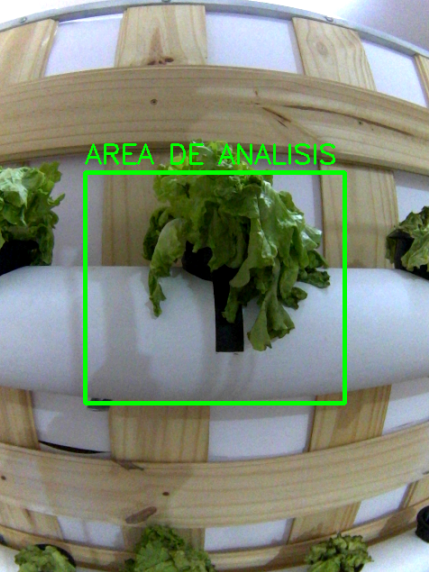
\includegraphics[width=0.75\textwidth]{imagenes/configuracion_cintas_referencia.png}
\caption{Disposición de cintas de referencia horizontal y vertical en el sistema hidropónico}
\label{fig:configuracion_cintas}
\end{figure}

\subsubsection{Metodología de Detección}

El algoritmo de detección de cintas explota el alto contraste entre el marcador negro y el fondo claro mediante procesamiento en el canal de valor (V) del espacio HSV. Esta elección se fundamenta en la invariancia del canal V ante cambios en la tonalidad cromática de la iluminación, propiedad demostrada en el marco teórico (Sección 2.2.1).

El proceso inicia con la captura de una imagen RGB de la región donde se espera encontrar el marcador. La imagen se transforma al espacio HSV aplicando las ecuaciones de conversión estándar, y se extrae el canal V que representa el brillo de cada píxel. Sobre este canal se aplica umbralización inversa con valor de referencia de 50, operación que asigna valor máximo (blanco) a los píxeles oscuros y valor nulo (negro) a los píxeles claros. Matemáticamente:

\begin{equation}
I_{bin}(x,y) = \begin{cases}
255 & \text{si } I_V(x,y) < 50 \\
0 & \text{si } I_V(x,y) \geq 50
\end{cases}
\end{equation}

El valor de umbral 50 se determinó empíricamente mediante análisis del histograma de intensidades en múltiples imágenes representativas, identificando el punto que maximiza la separación entre la distribución de intensidades de las cintas negras y la distribución de intensidades del fondo blanco.

Sobre la imagen binaria resultante se ejecuta el algoritmo de detección de contornos de Suzuki-Abe, obteniendo las fronteras de todas las regiones oscuras detectadas. Los contornos se filtran aplicando un criterio de área mínima de 500 píxeles, eliminando elementos espurios correspondientes a ruido o pequeñas sombras. Este umbral se estableció considerando que una cinta de 18 milímetros de ancho a 200 milímetros de distancia subtiende aproximadamente 120 píxeles de ancho en la imagen, resultando en áreas típicas superiores a 3000 píxeles para segmentos de cinta de longitud razonable.

\subsubsection{Evaluación de Calidad del Contorno}

Los contornos que superan el filtrado de área se someten a evaluación de calidad para discriminar entre cintas de referencia genuinas y otros elementos oscuros presentes en la escena (como plantas o vasos). La evaluación se basa en el análisis de la región basal del contorno, definida como el 10 por ciento inferior de su rectángulo delimitador.

Para cada contorno candidato se calcula su rectángulo delimitador $(x, y, w, h)$, donde $(x,y)$ representa la esquina superior izquierda, $w$ el ancho y $h$ la altura. La región basal se define entonces como:

\begin{equation}
R_{base} = \{(x',y') : x \leq x' < x+w, \, y+0.9h \leq y' < y+h\}
\end{equation}

Se calcula la fracción de píxeles blancos en esta región respecto al total de píxeles de la región:

\begin{equation}
Q_{base} = \frac{1}{|R_{base}|} \sum_{(x,y) \in R_{base}} \frac{I_{bin}(x,y)}{255}
\end{equation}

donde $|R_{base}|$ denota el número de píxeles en la región. Un valor $Q_{base}$ cercano a 1 indica que la región basal del contorno es consistentemente oscura, característica de las cintas de referencia cuyo borde inferior es nítido y bien definido. Valores inferiores indican contornos de objetos con bases irregulares o discontinuas, como plantas con hojas que no presentan un borde horizontal claro.

Esta métrica resulta efectiva para distinguir cintas de otros elementos oscuros: las cintas genuinas presentan típicamente $Q_{base} > 0.8$, mientras que plantas u otros objetos tienen $Q_{base} < 0.5$. Se establece un umbral de aceptación de 0.7 como compromiso entre sensibilidad y especificidad.

\subsubsection{Sistema de Scoring Multicriteria}

Cuando múltiples contornos cumplen los criterios de área mínima y calidad basal, se implementa un sistema de scoring ponderado que considera tres factores para seleccionar el mejor candidato.

El primer factor evalúa el área del contorno normalizada respecto a los límites mínimo y máximo esperados:

\begin{equation}
S_{área} = \frac{A - A_{min}}{A_{max} - A_{min}}
\end{equation}

donde $A$ es el área del contorno, $A_{min} = 500$ píxeles y $A_{max} = 50000$ píxeles. Este factor favorece contornos con áreas intermedias, descartando elementos excesivamente pequeños (ruido) o excesivamente grandes (probablemente no corresponden a una cinta individual).

El segundo factor evalúa la posición del centroide del contorno respecto al centro de la imagen:

\begin{equation}
S_{posición} = 1 - \frac{|c_x - x_{centro}|}{W_{imagen}/2}
\end{equation}

donde $c_x$ es la coordenada horizontal del centroide, $x_{centro}$ es la coordenada horizontal del centro de la imagen, y $W_{imagen}$ es el ancho total de la imagen. Este factor favorece contornos cercanos al centro, bajo la hipótesis de que el sistema de control posiciona aproximadamente el robot frente a la cinta objetivo, resultando en desviaciones pequeñas.

El tercer factor corresponde directamente a la calidad basal $Q_{base}$ calculada previamente, que favorece contornos con bordes inferiores bien definidos.

El score total se calcula como combinación lineal ponderada de estos tres factores:

\begin{equation}
S_{total} = w_1 \cdot S_{área} + w_2 \cdot S_{posición} + w_3 \cdot Q_{base}
\end{equation}

Los pesos se establecieron como $w_1 = 0.3$, $w_2 = 0.4$ y $w_3 = 0.3$, otorgando mayor importancia a la posición dado que las desviaciones típicas son inferiores a 50 milímetros, resultando en centroides próximos al centro de la imagen. El contorno con mayor score total se selecciona como la cinta de referencia.

\subsubsection{Cálculo de Desviación}

Una vez identificado el contorno óptimo se procede al cálculo de la desviación espacial. Se determina el centroide del contorno mediante sus momentos de imagen:

\begin{equation}
c_x = \frac{M_{10}}{M_{00}}, \quad c_y = \frac{M_{01}}{M_{00}}
\end{equation}

La desviación en píxeles se calcula como la diferencia entre las coordenadas del centroide y las coordenadas del centro de la imagen:

\begin{equation}
\Delta x_{px} = c_x - \frac{W_{imagen}}{2}
\end{equation}

\begin{equation}
\Delta y_{px} = c_y - \frac{H_{imagen}}{2}
\end{equation}

Para una imagen de 1920×1080 píxeles, el centro se ubica en (960, 540). Un centroide detectado en (1100, 540) resultaría en $\Delta x_{px} = 140$ píxeles, indicando que el robot se encuentra desplazado 140 píxeles hacia la izquierda respecto a la posición ideal.

Estas desviaciones en píxeles se convierten posteriormente a milímetros mediante los coeficientes de calibración, proceso que se detalla en la siguiente sección.

\subsubsection{Discriminación de Orientación}

Para determinar si un contorno detectado corresponde a una cinta horizontal o vertical se analiza la relación de aspecto de su rectángulo delimitador. Esta relación se define como:

\begin{equation}
AR = \frac{w}{h}
\end{equation}

donde $w$ y $h$ son el ancho y altura del rectángulo delimitador. Cintas horizontales, al tener su dimensión principal en dirección horizontal, presentan $AR > 2$. Cintas verticales, con su dimensión principal en dirección vertical, presentan $AR < 0.5$. Contornos con relaciones de aspecto intermedias ($0.5 \leq AR \leq 2$) se consideran ambiguos y se descartan.

Este análisis permite al sistema identificar automáticamente el tipo de cinta detectada, información necesaria para interpretar correctamente la desviación calculada. Una desviación horizontal del centroide respecto al centro indica desplazamiento en X cuando se detecta una cinta vertical, o desplazamiento en Y cuando se detecta una cinta horizontal.

\subsubsection{Desempeño del Algoritmo}

El tiempo de ejecución promedio del algoritmo completo de detección de cintas es de 95 milisegundos, desglosado en: conversión al espacio HSV (15 ms), extracción del canal V (2 ms), umbralización (8 ms), detección de contornos (30 ms), filtrado inicial (5 ms), evaluación de calidad basal (20 ms), cálculo de scores (10 ms), y determinación del centroide (5 ms).

Esta latencia permite una frecuencia de actualización de aproximadamente 10 Hz, suficiente para compensar errores de posicionamiento durante el movimiento del robot a velocidades de 5 a 10 cm/s. En pruebas de validación con 200 imágenes de cintas bajo diferentes condiciones de iluminación, el algoritmo alcanzó una tasa de detección correcta del 97.5 por ciento, con fallos principalmente en casos de iluminación extremadamente baja (inferior a 400 lux) donde el contraste se reduce significativamente.